\documentclass{beamer}

\usepackage{graphicx}

\title{Week 2 CUSF Controls Introductory Project - Modelling Principles and State Space}
\author{Yoonjae Hwang}
\date{19 October 2025}

\begin{document}

\frame{\titlepage} 
\begin{frame}
\frametitle{Motivation - why do we need models?}
\begin{itemize}
    \item Models are mathematical representation of a system
    \item We can answer questions without physical experimenting with analysis and simulations
    \item Models are fundamentally approximations of reality
    \item The fidelity of the model comes at the cost of complexity, and it is the engineer's decision which model to choose
\end{itemize}
\end{frame}

\begin{frame}
\frametitle{Mechanics}
The dynamics of many systems can be described by its equations of motion (EoMs). 
We can derive the EoMs using various approaches (Newton, Lagrange, Hamiltonian)

\begin{equation}
    F = ma
\end{equation}

\begin{equation}
    \frac{d}{dt} \left( \frac{\partial \mathcal{L}}{\partial \dot{q_i}} \right)- \frac{\partial \mathcal{L}}{\partial q} = 0
\end{equation}

\begin{equation}
    \frac{dq}{dt} = \frac{\partial \mathcal{H}}{\partial p}, \frac{dp}{dt} = -\frac{\partial \mathcal{H}}{\partial q}
\end{equation}
\end{frame}


\begin{frame}
\frametitle{Electrical Engineering Perspective - Input/Output Systems}
\begin{columns}
\begin{column}{0.5\textwidth}
\begin{itemize}
    \item Systems takes in inputs, and produces outputs
    \item This way, we decompose complex systems as many systems connected together
    \item Particularly useful for Linear Time-Invariant Systems (LTI)
    \item Step-response, impulse response and frequency response
\end{itemize}   
\end{column}

\begin{column}{0.5\textwidth}
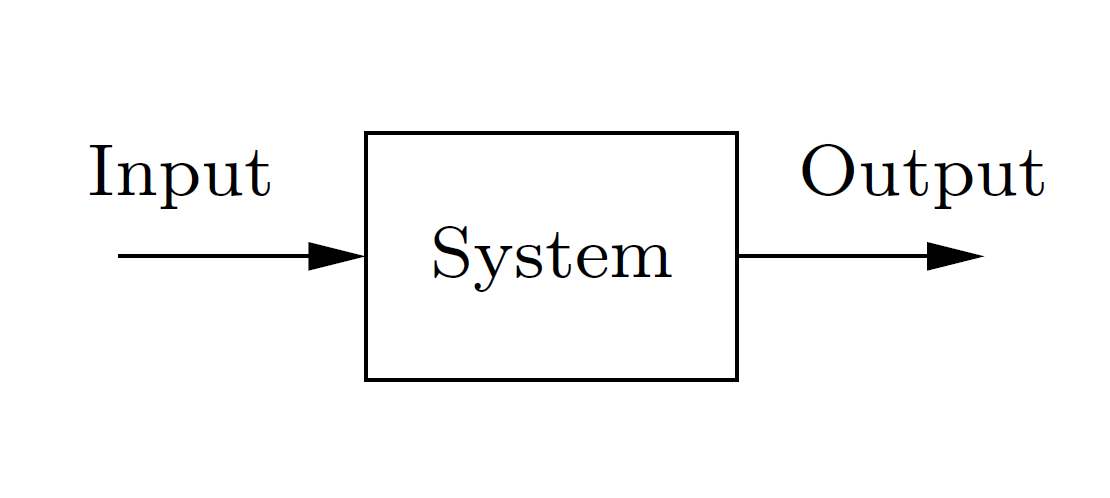
\includegraphics[width = \textwidth]{InputOutput.png}
\end{column}
\end{columns}

\end{frame}


\begin{frame}
\frametitle{Dynamic Modelling - State Space Representation}
Whichever approach, we often end up with some differential equation.
Most of the times, we are dealing with Ordinary Differential Equations:
\begin{equation}
    \dot{x} = f(x, u, t), \qquad y = h(x, u, t)
\end{equation}

\begin{itemize}
    \item $x \in \mathbb{R}^n$ and $u \in \mathbb{R}^m$ are state and input vectors. 
    \item Each component of the vectors are the different variables that describe the system
    \item The dimension of the state vector is the order of the system
    \item If the functions $f, h$ do have any time dependence, then we say the system is time-invariant
\end{itemize}

\end{frame}

\begin{frame}
\frametitle{Linear State Space Models}
Often, we will find ourselves working with systems where the functions $f,h$ are linear in $x$ and $u$.
Then, the system can be described with matrices A, B, C, D as such: 
\begin{equation}
    \dot{x} = A x + Bu \qquad y = Cx + Du
\end{equation}
\begin{itemize}
    \item This is the general representation for LTI systems
    \item A, the dynamics matrix, represents the dynamics of the autonomous system
    \item B, the control matrix, tells how the input variables are related to the state variables
    \item C is the sensor matrix, as it tells us the relationship between what we can measure directly and the internal states
    \item D is the direct term -  we don't see this often
\end{itemize}
\end{frame}

\begin{frame}
\frametitle{Linear State Space Models}
If we generalise LTI single-input single-output systems (SISO), we have: 
\begin{equation}
    \frac{d^n y}{dt^n} + a_1 \frac{d^{n-1}y}{dt^{n-1}} + \dots + a_n y = u
\end{equation}

To convert this into state space form, we define the state to be: 
\begin{equation}
x = 
\begin{pmatrix}
x_1 \\[4pt]
x_2 \\[4pt]
\vdots \\[4pt]
x_{n-1} \\[4pt]
x_n
\end{pmatrix}
=
\begin{pmatrix}
\dfrac{d^{n-1}y}{dt^{n-1}} \\[6pt]
\dfrac{d^{n-2}y}{dt^{n-2}} \\[6pt]
\vdots \\[6pt]
\dfrac{dy}{dt} \\[6pt]
y
\end{pmatrix}
\end{equation}

\end{frame}

\begin{frame}
\frametitle{Linear State Space Models}
Then, the state space equations then become: 
\begin{equation}
\frac{d}{dt}
\begin{pmatrix}
x_1 \\[4pt]
x_2 \\[4pt]
\vdots \\[4pt]
x_{n-1} \\[4pt]
x_n
\end{pmatrix}
=
\begin{pmatrix}
 -a_1 x_1 - \cdots - a_n x_n \\[4pt]
 x_1 \\[4pt]
 \vdots \\[4pt]
 x_{n-2} \\[4pt]
 x_{n-1}
\end{pmatrix}
+
\begin{pmatrix}
u \\[4pt]
0 \\[4pt]
\vdots \\[4pt]
0 \\[4pt]
0
\end{pmatrix},
\qquad
y = x_n.
\end{equation}
We'll go through some examples.
\end{frame}

\begin{frame}
\frametitle{Transfer Functions}
In many practical situations, one can model the input/output of a system using equations of the form: 
\begin{equation}
\frac{d^n y}{dt^n} + a_1 \frac{d^{n-1} y}{d t^{n-1}} + \dots + a_n y = b_0 \frac{d^m u}{d t^m} + \dots + b_m u
\end{equation}

The characteristic polynomials are then given by (assuming they dont have common roots): 
\begin{equation}
    a(s) = s^n + a_1 s^{n-1} + \dots + a_n, \qquad b(s) = b_0 s^m + \dots b_m
\end{equation}
$s$ is a complex number, and can be represented by $\sigma \pm j \omega$. 
\end{frame}

\begin{frame}
\frametitle{Transfer Functions}
The general solution to the homogenous equation which does not depend on the input, are given by: 
\begin{equation}
    y(t) = \sum_{k=1}^{n} C_k e^{s_k t}
\end{equation}
If there are repeated roots: 
\begin{equation}
    y(t) = \sum_{k=1}^{n} C_k(t) e^{s_k t}
\end{equation}
\end{frame}

\begin{frame}
\frametitle{Transfer Functions}
Now we consider the particular integral. 
\newline
Upon an input $u(t) = e^{st}$, where $s \neq s_k$, we investigate solutions of the form: 
$y(t) = G(s)e^{st}$.
Differentiating $u$ and $y$ with respect to time sufficiently many times, and substituting back into the original differential equation we obtain: 
\begin{equation}
    (s^n + a_1 s^{n-1} + \dots + a_n) G(s) e^{st} = (b_0 s^m + b_1 s^{m-1} + \dots + b_m) e^{st}
\end{equation}
Hence
\begin{equation}
    G(s) = \frac{b_0 s^m + b_1 s^{m-1} + \dots + b_m}{s^n + a_1 s^{n-1} + \dots + a_n}
\end{equation}
$G(s)$ is called the transfer function of the system
\end{frame}

\begin{frame}
\frametitle{Laplace Transforms and Transfer Functions}
The Laplace Transform is an integral transform that converts the states from the time-domain to the s-domain. 
\begin{equation}
    \mathcal{L}[f(t)] = \int_{0}^{\infty} f(t) e^{-st} dt
\end{equation}
The numerator and denominator of the transfer function are then the Laplace Transform of the output and input states:
\begin{equation}
    G(s) = \frac{Y(s)}{U(s)}
\end{equation}
You will study Laplace Transforms in more detail in IA maths in Easter. 
Using transfer functions, decribing how different systems connect becomes much easier. 
\end{frame}


\end{document}